\problemname{Bulldozer}

You are tasked with bulldozing some buildings that stand along a long,
straight road. The buildings are modelled as evenly spaced stacks of
identical square blocks along an infinite line.  Your powerful
bulldozer is capable of moving any one of these blocks one unit of
distance to the left or to the right. This may push other blocks out of the way, and
blocks which sit atop moving blocks will move along. Blocks which are
pushed over a gap fall down until they reach either the ground or
another block.

For instance, consider the stacks of blocks shown on the left in
Figure~\ref{fig:bulldozer} below.  If you push the block labelled C to
the right, the blocks D and E would be pushed along to the
right, since they are in the way. Blocks A, B and F would
also move along because they are sitting on top of moving blocks. After
pushing C to the right, E would be sitting over a gap, so
E and F drop down to fill that gap. The resulting stacks
are shown in the middle of Figure~\ref{fig:bulldozer}.  Pushing block
C one further step to the right would result in the configuration
shown on the right.

Your goal is to \emph{level} all the buildings: bulldoze until all
stacks are of height at most $1$, i.e., all blocks are on the ground.
Note that the road stretches out infinitely far on either side, so
this is always possible.

Given the initial heights of the stacks, determine the smallest number
of moves you need to make to level all the buildings, where a move
consists of using the bulldozer to push one block one step to the left
or right.

\begin{figure}[!h]
    \centering
    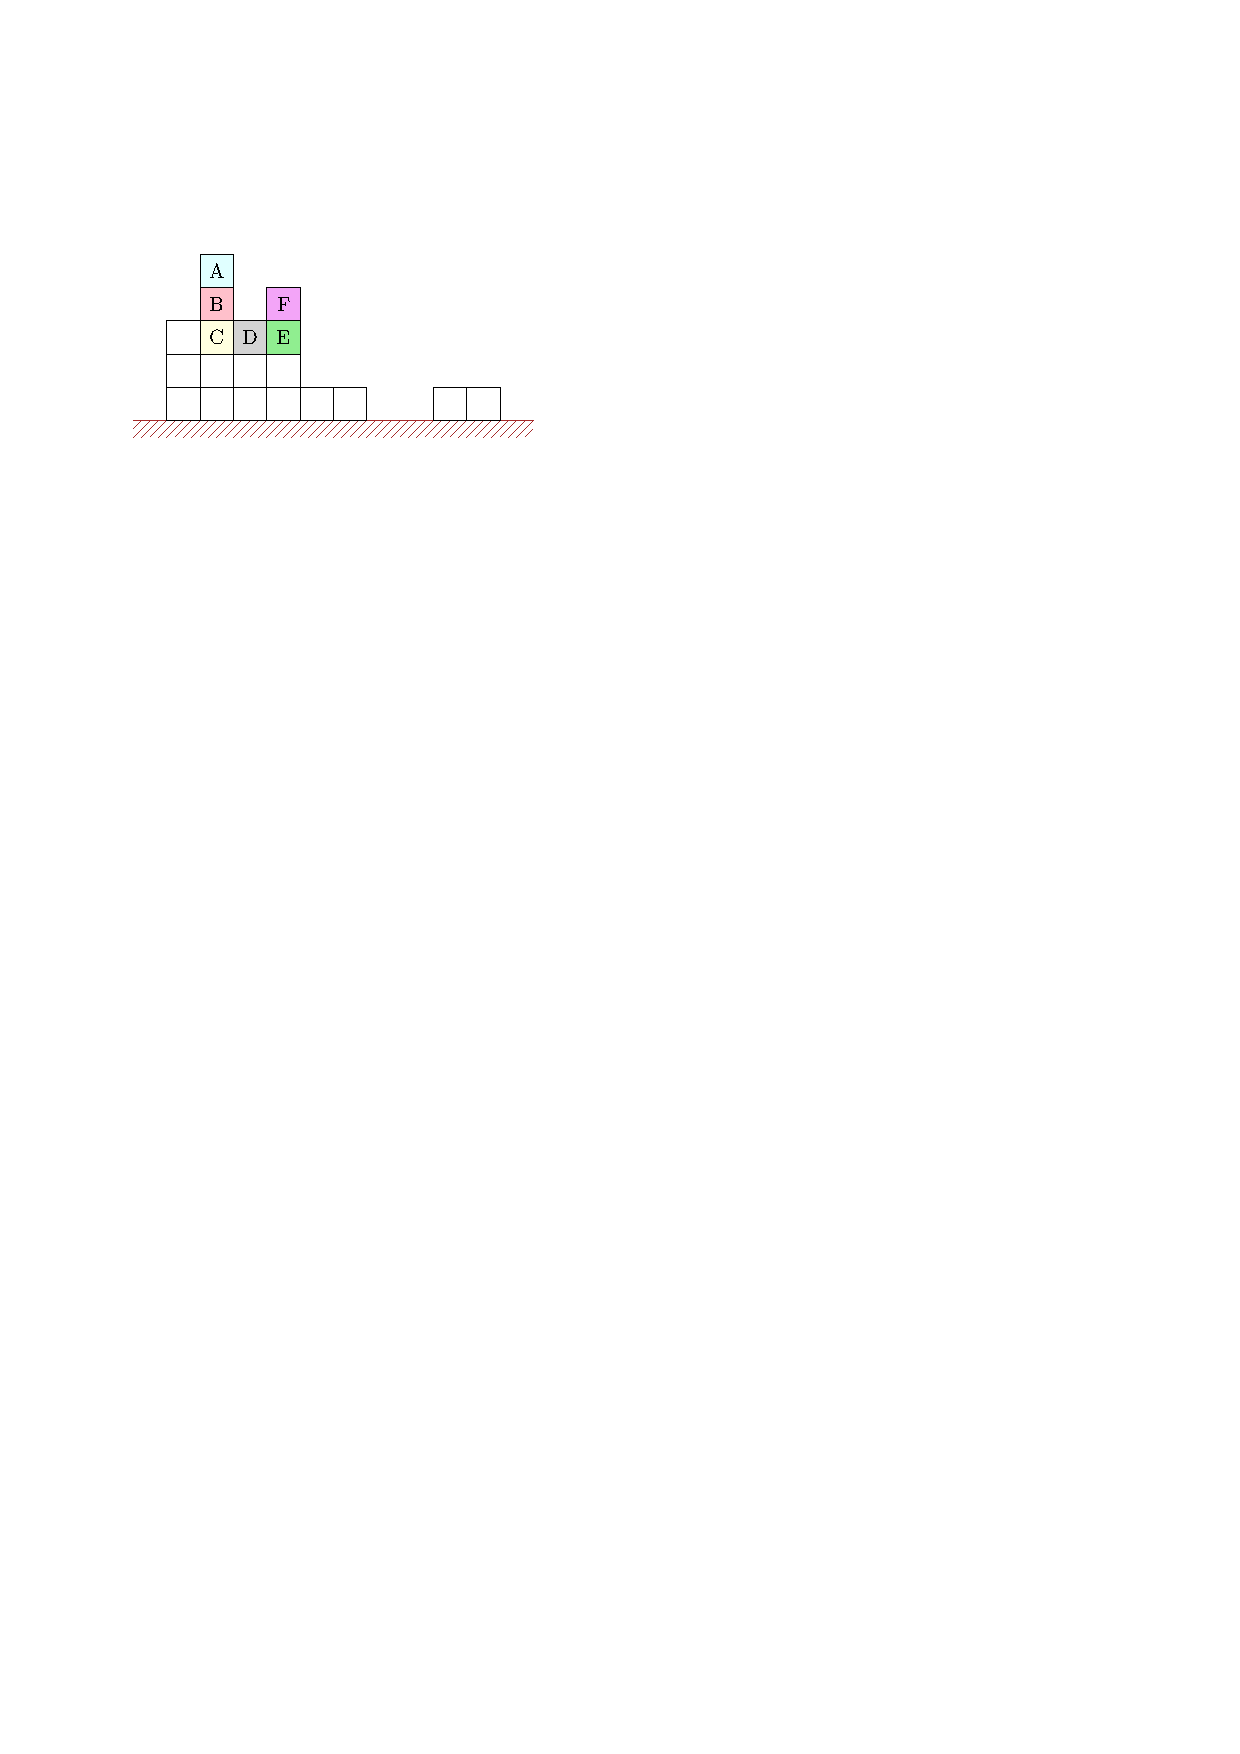
\includegraphics[width=0.3\textwidth]{fig1}
    \quad
    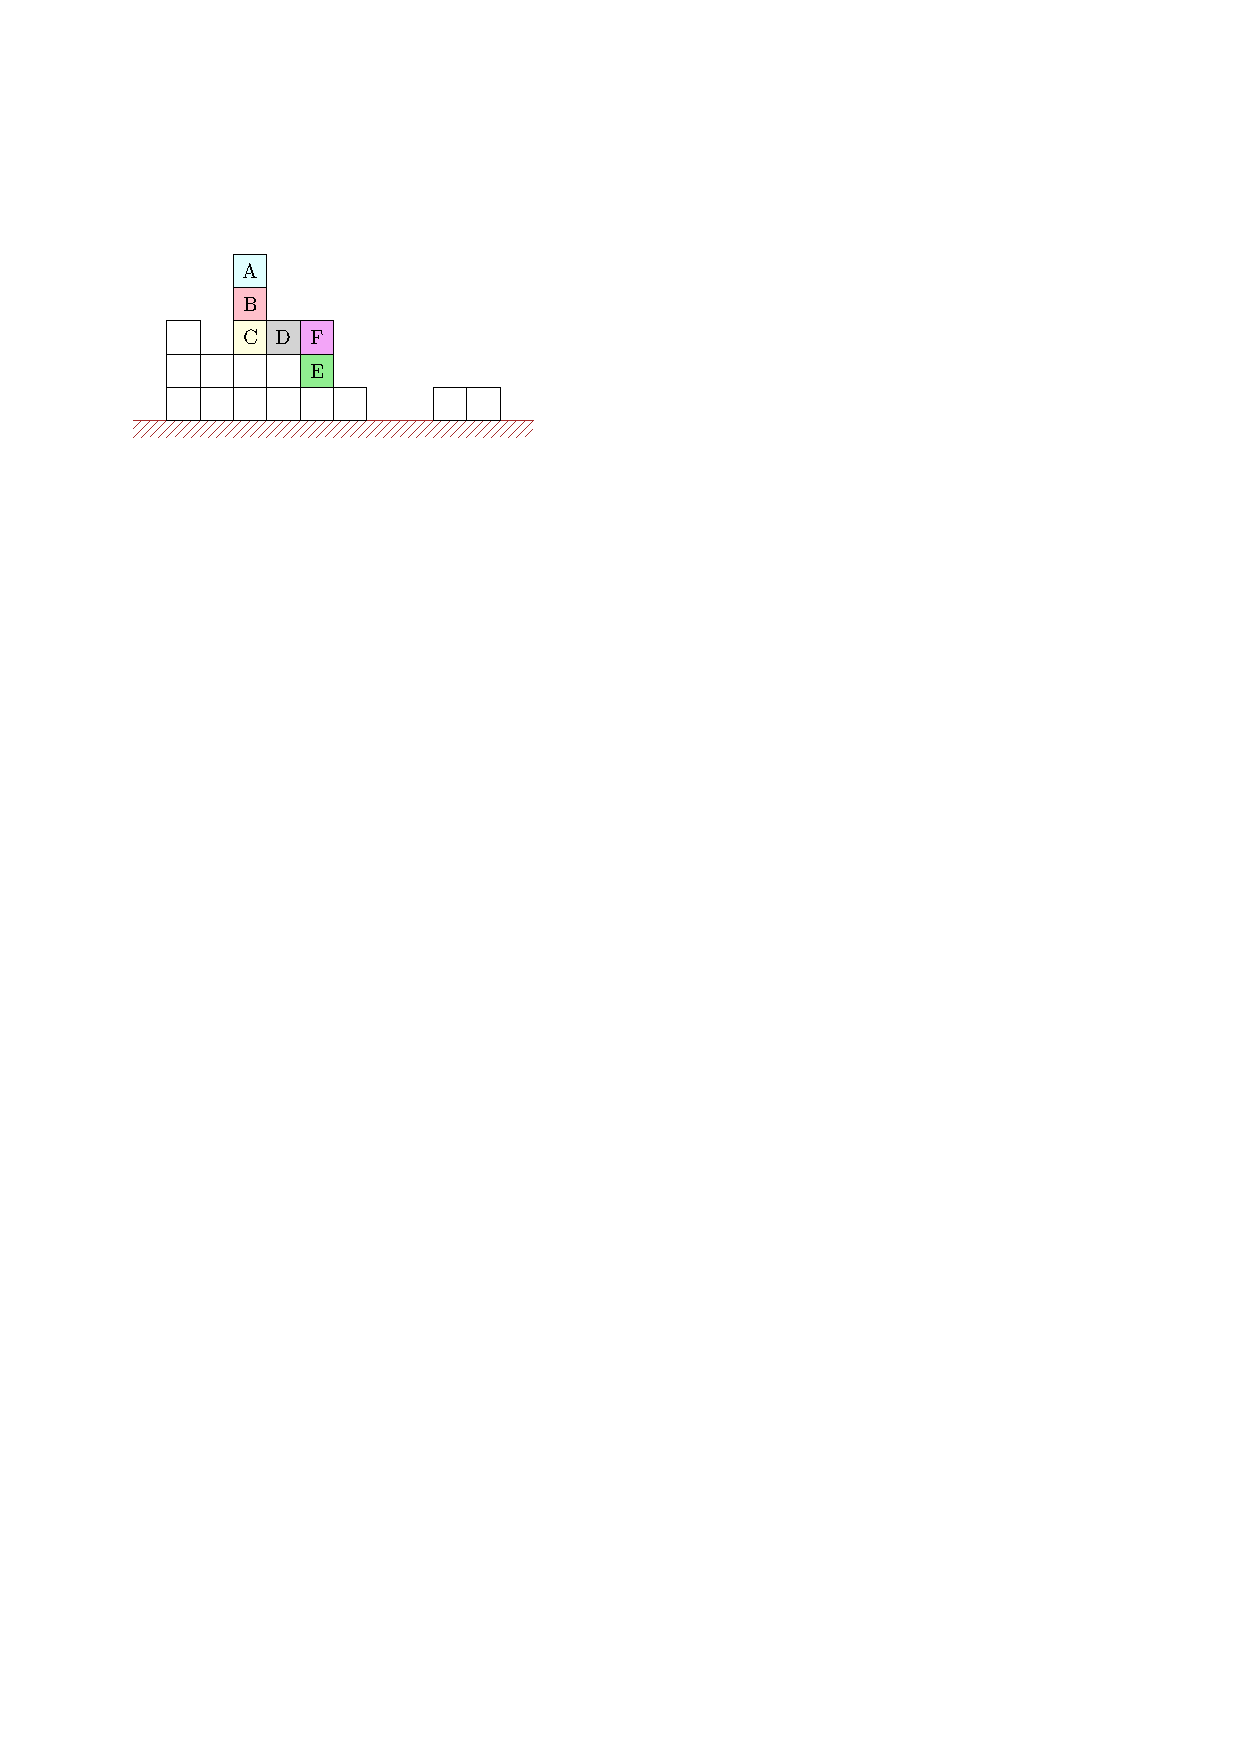
\includegraphics[width=0.3\textwidth]{fig2}
    \quad
    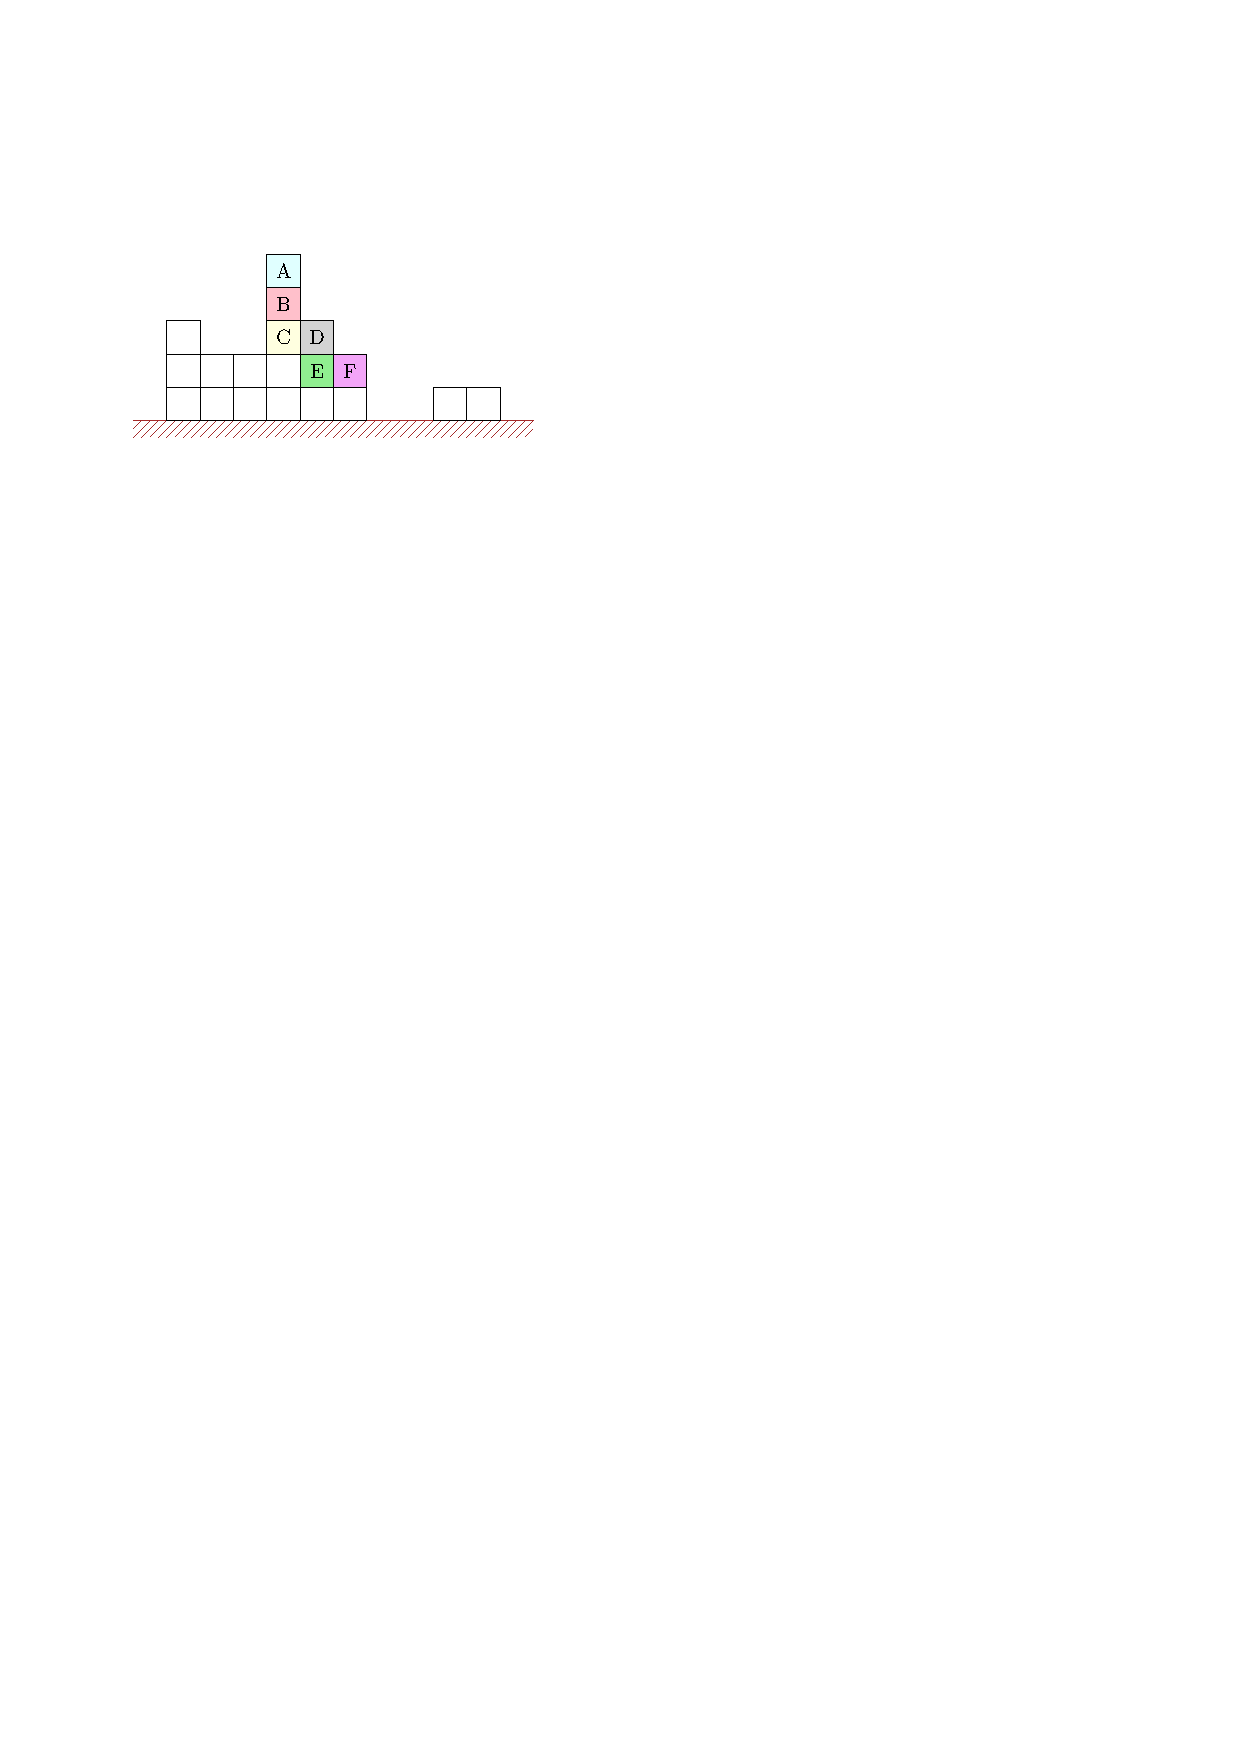
\includegraphics[width=0.3\textwidth]{fig3}
    \caption{Illustration of a configuration of stacks of blocks, and the results of pushing the block labelled C towards the right twice (the blocks labelled A--F are coloured and labelled only for illustrative purposes).}
    \label{fig:bulldozer}
\end{figure}


\begin{Input}
The input consists of:

\begin{itemize}
\item One line with an integer $n$ ($1 \le n \leq 2 \cdot 10^5$), the number of stacks of blocks.
\item One line with $n$ integers $a_1, \ldots, a_n$ ($0 \leq a_i \leq 10^9$ for each $i$), the
  initial heights of the stacks from left to right.
\end{itemize}

The example shown on the left in Figure~\ref{fig:bulldozer} could be
given by $3, 5, 3, 4, 1, 1, 0, 0, 1, 1$, but it could also be left- or
right-padded with additional zeros.
\end{Input}

\begin{Output}
Output the minimum number of moves required to level every building.
\end{Output}

